\documentclass[10pt]{beamer}
\usetheme{Boadilla} % My favorite!
\setbeamercovered{invisible}
% To remove the navigation symbols from 
% the bottom of slides%
\setbeamertemplate{navigation symbols}{} 
\setbeamertemplate{itemize items}[default]
\setbeamertemplate{enumerate items}[default]
\xdefinecolor{lavendar}{rgb}{0.2, 0.2, 0.72}
%
\usepackage{graphicx,epsfig}

%\usepackage{bm}         % For typesetting bold math (not \mathbold)
%\logo{\includegraphics[height=0.6cm]{yourlogo.eps}}
%
\newcommand{\be}{\begin{equation*}}
\newcommand{\ee}{\end{equation*}}
\newcommand{\ba}{\begin{eqnarray}}
\newcommand{\ea}{\end{eqnarray}}

\newcommand{\vso}{\vskip15pt}
\newcommand{\vst}{\vskip30pt}
\newcommand{\nsub}{n_\mathrm{sub}}

\def\smallfrac#1#2{\hbox{${{#1}\over {#2}}$}}

\title[]{Impact of LHC data on (NN)PDFs}
\author{Nathan Hartland}
\institute
{
University of Edinburgh\\
%\includegraphics[height=2cm]{edinburghcrest.pdf}
\medskip
}
% \today will show current date. 
% Alternatively, you can specify a date.
%

\date{\today}


\begin{document}
\renewcommand{\inserttotalframenumber}{14}


\begin{frame}
\begin{centering}
\vskip20pt
\center{\huge\color{lavendar} \textbf{Impact of LHC data on (NN)PDFs}}
\vskip20pt
Nathan Hartland\\

\small{The University of Edinburgh}\\
\vso
\includegraphics[height=2cm]{edinburghcrest.pdf}

\vskip10pt
{\bf The NNPDF Collaboration:}\\
R.~D.~Ball, V.~Bertone, F.~Cerutti,
C.~Deans, L.~Del~Debbio, \\S~Forte,
A~Guffanti, N.H, J.I.~Latorre, J.~Rojo and M.~Ubiali. 
\vskip20pt
XLVInd Rencontres de Moriond\\
La Thuile, Aosta valley, Italy\\
March 10th -March 17th, 2012


\end{centering}

\end{frame}

\section{Parton distribution fitting}
\begin{frame}
\frametitle{Parton distributions for the LHC}
\be \sigma_X= \sum_{a,b} \int_0^1 dx_1dx_2 f_a(x_1,Q^2)f_b(x_2,Q^2)\sigma_{q_aq_b \to X} \left( x_1,x_2,Q^2 \right) \ee
\begin{itemize}
		\item<1-> Need to have a reliable determination of PDFs for LHC physics.
		\item<1-> An accurate estimation of PDF uncertainties is crucial.
\end{itemize}

\begin{columns}
  \begin{column}{0.45\textwidth}
      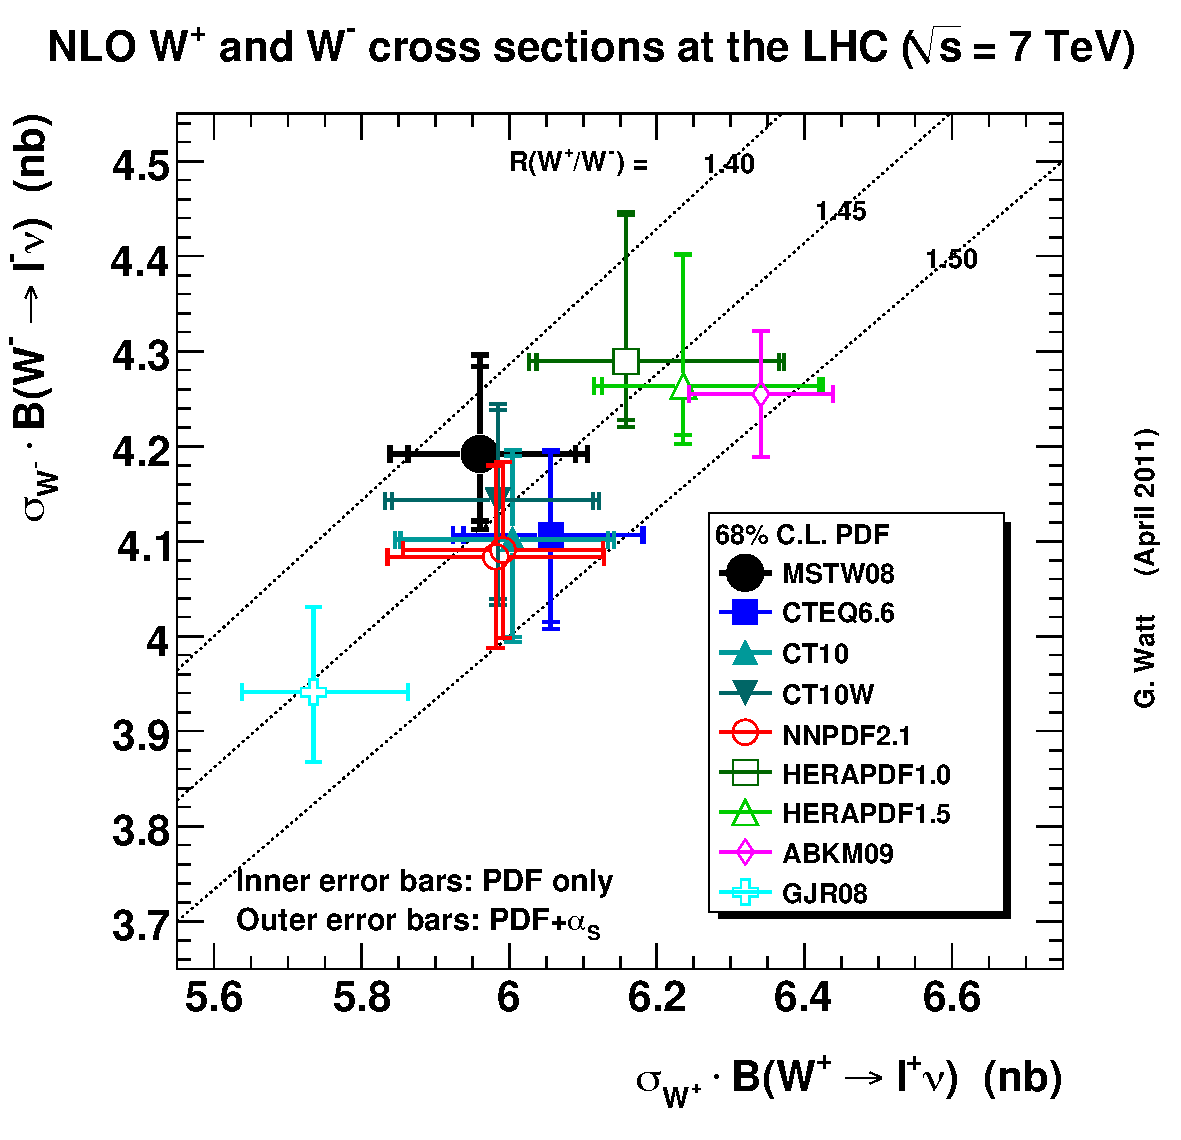
\includegraphics[width=1.0\textwidth]{w+w-lhc7nlo68err.eps}
  \end{column}
  
    \begin{column}{0.55\textwidth}
      \includegraphics[width=1.0\textwidth]{ratiogglumi1_68cl.eps}\\
      \quad { \centering \quad\quad \small \color{blue} G. Watt [hep-ph/1106.5788]}\\

  \end{column}  
  \end{columns}

\end{frame}

\begin{frame}
\frametitle{NNPDF approach to parton fitting}
\begin{itemize}
\item<1->Use of Neural Networks as unbiased and extremely flexible interpolators.
\begin{itemize}
\item<1->Each PDF has 37 free parameters to vary in the fit.
\item<1->Total of 259 free parameters minimises parametrisation bias.
\end{itemize}

\item<1->Monte Carlo approach to uncertainty estimation.
\begin{itemize}
\item<1->Perform an independent NN fit upon an ensemble of artificial data sets.\\
\item<1->Ensemble of PDF replicas faithfully represent the uncertainty in the original experimental data without the need for a tolerance criterion.
\end{itemize}
\end{itemize}
\begin{columns}
  \begin{column}{0.25\textwidth}
		\be \langle\mathcal{O}\rangle=\smallfrac{1}{N}\,\sum_{k=1}^{N}\mathcal{O}[f_k]\, .\ee
  \end{column}
  
    \begin{column}{0.4\textwidth}
		\be {\mathrm{Var}}[\mathcal{O}]=\smallfrac{1}{N}\,\sum_{k=1}^{N}(\mathcal{O}[f_k] -  \langle\mathcal{O}\rangle )^2 .\ee
  \end{column}  
  \end{columns}

 \begin{figure}[b!]
    \begin{center}
      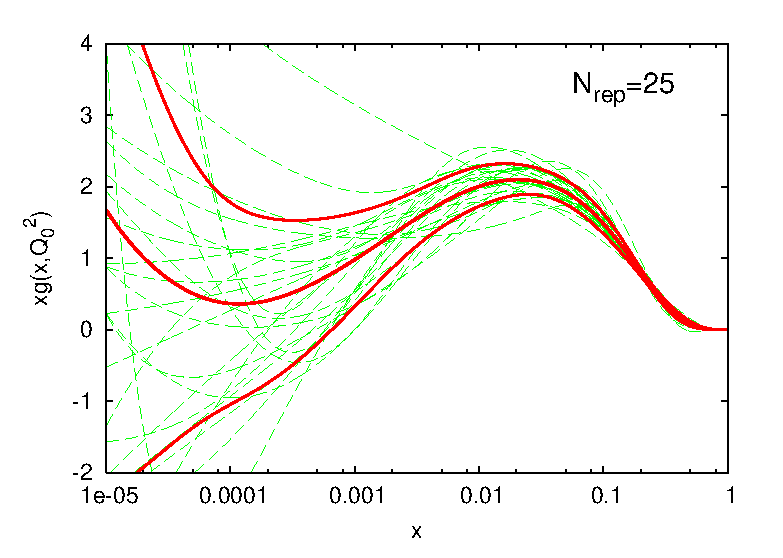
\includegraphics[width=0.45\textwidth]{glureplicas25.eps}
      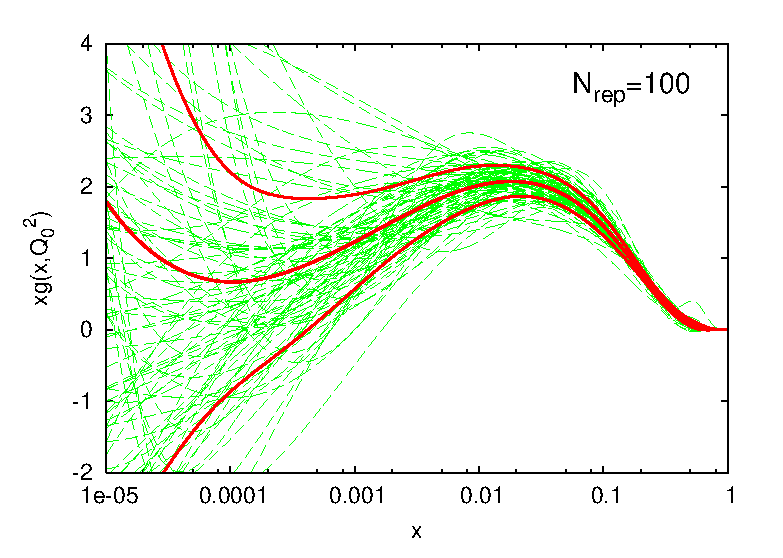
\includegraphics[width=0.45\textwidth]{glureplicas100.eps}
    \end{center}
    \vskip-0.5cm
    \label{fig:pdf-jets}
\end{figure}


\end{frame}

\begin{frame}
\frametitle{ NNPDF collider only fits }

\underline{Target}: An NNPDF Fit based only upon collider data
\begin{itemize}
\item<1-> Free of contamination from higher twists.
\item<1-> No nuclear corrections required.
\end{itemize}

 \begin{figure}[b!]
    \begin{center}
      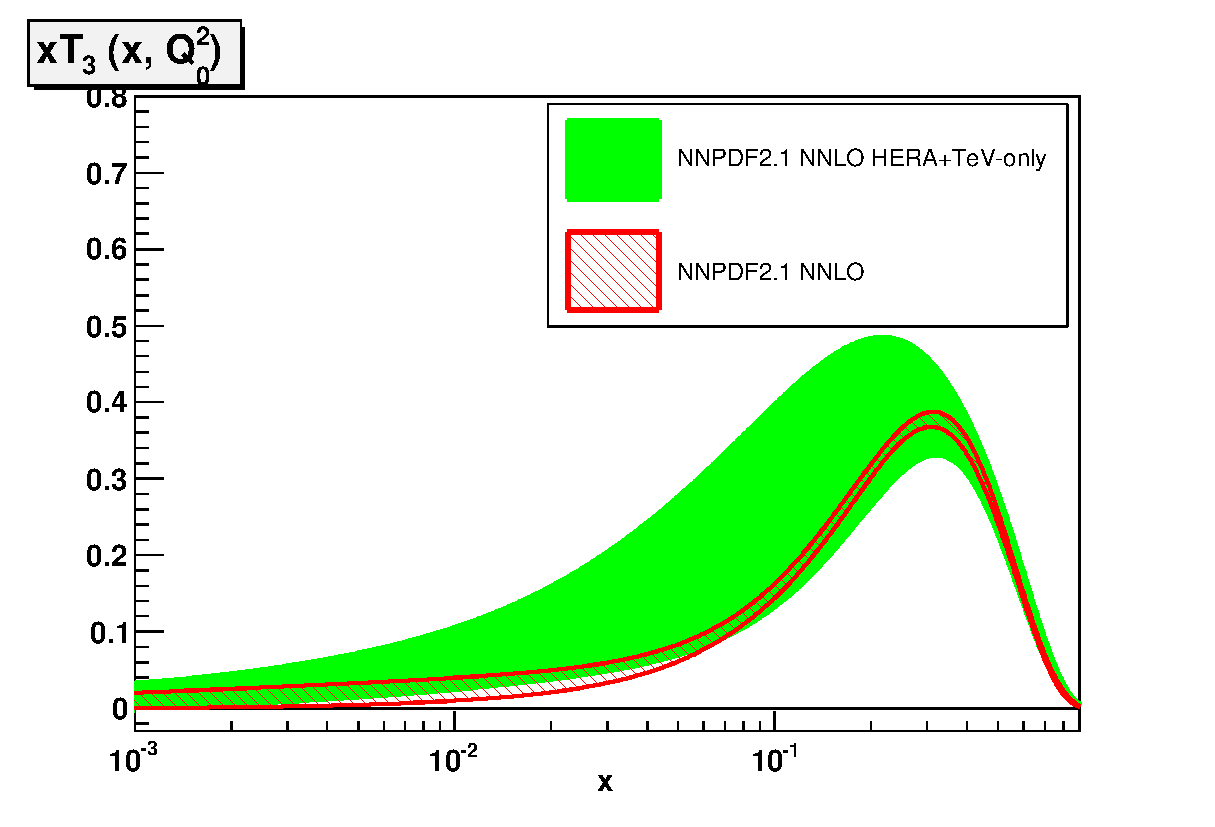
\includegraphics[width=0.50\textwidth]{xT3_Q_2_log-nnpdf21nnlo-collider.eps}
      \includegraphics[width=0.50\textwidth]{xSinglet_Q_2_log-nnpdf21nnlo-collider.eps}
    \end{center}
    \vskip-0.5cm
    \label{fig:pdf-jets}
\end{figure}
\begin{itemize}
\item<1->HERA + Tevatron data provide insufficient constraints in an NNPDF fit
\end{itemize}

\begin{itemize}
\item<1-> LHC data will be crucial to properly constrain future collider only NNPDFs
\end{itemize}
\end{frame}

\begin{frame}
\frametitle{Including new experimental data}
How can we add new LHC data to an existing parton set?

\begin{itemize}
		\item<1-> Full Refit\\
\end{itemize}
\underline{Tools}: APPLgrid/FastNLO projects $\to$ MC Weights on an interpolation grid
\be W = \sum_p \sum_{l=0}^{\nsub} \sum_{i_{y_1}} \sum_{i_{y_2}} \sum_{i_\tau}
W_{i_{y_1},i_{y_2},i_\tau}^{(p)(l)} \, \left( \frac{\alpha_s\left({Q^2}^{(i_\tau)}\right)}{2\pi}\right)^{p}
F^{(l)}\left(x_1^{(i_{y_1})}, x_2^{(i_{y_1})},  {Q^2}^{(i_\tau)}\right)
\ee
Fast ... but can we get faster? $\to$ combine weight tables with FastKernel evolution:
\be E^\tau_{\alpha\beta j k} = \int_{x_\alpha}^1 \frac{dy}{y}\Gamma_{ij}\left( \frac{x_\beta}{y},Q_0^2,Q_\tau^2 \right) \mathcal{I}^{(\beta)}(y). \ee
\be f_i(x_{\alpha},Q^2_\tau) =  \sum_j^{N_{\mathrm{pdf}}}R_{ij}N_j(x_{\alpha},Q_\tau^2) = \sum_{\beta}^{N_x}  \sum_{j,k}^{N_{\mathrm{pdf}}} R_{ij}E^\tau_{\alpha\beta jk}N^0_k(x_\beta).\ee 

\begin{columns}
  \begin{column}{0.6\textwidth}
Combined Weight-Evolution tables
\begin{itemize}
		\item<1-> More of the calculation is precomputed\\
		\item<1-> Smaller flavour basis at initial scale\\
\end{itemize}  \end{column}
    \begin{column}{0.4\textwidth}
 % \begin{block}{}
  \be W= \sum_{\alpha,\beta}^{N_x}\sum_{i,j}^{N_{\mathrm{pdf}}} \sigma_{\alpha\beta i j}N_i^0(x_\alpha)N_j^0(x_\beta)\ee
%\end{block}

	  \end{column}
  \end{columns}


  
  
\end{frame}

\begin{frame}
\frametitle{Including new experimental data}
How can we add new LHC data to an existing parton set?

\begin{itemize}
		\item<1-> Full Refit $\to$ Work in progress!
		\item<1-> Reweight existing Monte Carlo parton set. {\small \color{blue} Giele, Keller [hep-ph/9803393] }\\
\end{itemize}
If the new data is statistically independent of the data in the prior set:
\be
\mathcal{P}_{\rm new}(f)
= \mathcal{N}_{\chi}\mathcal{P}(\chi^2|f)\;\mathcal{P}_{\rm old}(f),
\ee
		\be \langle\mathcal{O}\rangle_{\mathrm {new}}=\int \mathcal{O}[f] \, \mathcal{P}_{ \mathrm {new}}(f)\,Df=\smallfrac{1}{N}\,\sum_{k=1}^{N}w_k\mathcal{O}[f_k].\,  \ee
Weights determined by statistical inference
\be w_k =\mathcal{N}_\chi\mathcal{P}(\chi^2|f_k) = 
\frac{(\chi^{2}_k)^{(n-1)/2} 
e^{-\frac{1}{2}\chi^{2}_k}}
{\smallfrac{1}{N}\sum_{k=1}^{N}(\chi^{2}_k)^{(n-1)/2}
e^{-\frac{1}{2}\chi^{2}_k}}\, .\ee
 Number of effective replicas reduced after reweighting: \be N_{\textrm{ eff}} \equiv \exp \left(\frac{1}{N_{\mathrm{rep}}}\sum_{k=1}^{N_{\mathrm{rep}}}w_k\ln(N_{\mathrm{rep}}/w_k)\right)\ee
\center{ \small  R.~D.~Ball {\it et al.} Nucl.\ Phys.\ B {\bf 849} 112  {\color{blue} [arXiv:1012.0836]}. }


\end{frame}

\begin{frame}
\frametitle{Application: NNPDF2.2 Parton Set .}
New data added by reweighting NNPDF2.1 Fit: $W$ leptonic charge asymmetry.
\begin{centering}
\center{\small  R.~D.~Ball {\it et al}, Nucl.\ Phys.\ B {\bf 855} 608 {\color{blue} [arXiv:1108.1758] }.}\\
\end{centering}\vskip5pt
Defined in terms of $W^{\pm}\to l^\pm\nu_l $ differential cross-sections $d\sigma_{l^\pm}/d\eta_l$
\be 
  A^l_W=\frac{d\sigma_{l^{+}}/d\eta_{l}-d\sigma_{l^{-}}/d\eta_{l}}
  {d\sigma_{l^{+}}/d\eta_{l}+d\sigma_{l^{-}}/d\eta_{l}}, 
\ee

\begin{itemize}
		\item<1-> ATLAS $\mu$ charge asymmetry. \hspace*{\fill {  \color{blue} [arXiv:1103.2929]}}
		\item<1-> CMS $e+\mu$ charge asymmetry. \hspace*{\fill { \color{blue}  [arXiv:1103.3470] }}
		\item<1-> D0 $e+\mu$ charge asymmetry. \hspace*{\fill { \color{blue} [arXiv:0709.4254]}}
\end{itemize}

\begin{figure}[h!]
  \centering
  \epsfig{width=0.44\textwidth,figure=xu-nnpdf22.eps}
  \epsfig{width=0.44\textwidth,figure=xd-nnpdf22.eps}
\end{figure}

\end{frame}

\begin{frame}
\frametitle{Updated LHC Data}
\begin{itemize}
\item<1-> LHC data in NNPDF2.2 now superseded
 \begin{itemize}
 \item<1-> Full covariance matrix available for the ATLAS W and Z rapidity distributions.
  \item<1-> Higher integrated luminosity 234 pb$^{-1}$ data for CMS muon asymmetry.
\end{itemize}
\end{itemize}

\begin{itemize}
\item<1-> Additional LHC Data
\begin{itemize}
\item<1-> $36$ pb$^{-1}$ Inclusive jet measurements (Full covariance matrix for ATLAS).
\item<1-> $36$ pb$^{-1}$ LHCb Z rapidity distribution, W lepton asymmetry. 
\item<1-> {\color{blue}$840$pb$^{-1}$ CMS  W electron asymmetry with full covariance matrix.}
\item<1-> {\color{blue}$4.67$fb$^{-1}$ CMS Inclusive jet measurement.}
\end{itemize}
\end{itemize}
\vso
\begin{centering}
\textbf { \footnotesize $\chi^2$ to electroweak vector boson production data}\\
\end{centering}
\begin{table}[h]
\scriptsize
\begin{center}
\begin{tabular}{|c|c|c|c|c|c|}
\hline
Dataset  , $\chi^2$ &  NNPDF2.1  &  MSTW08 & ABKM09  
& JR09 & HERAPDF1.5      \\  
\hline
\hline
ATLAS W/Z Rapidity  & 2.7    & 3.6 & 3.6 & 5.0 & 2.0\\
\hline
CMS $\mu$ asym  + Z Rap  & 2.0   & 3.0 & 2.8 & 3.6& 2.8\\  
\hline
LHCb W asym + Z Rap     & 0.8   & 0.7 & 1.2 & 0.4& 0.6\\
\hline
\end{tabular}
\end{center}
\end{table}
\begin{centering}
\textbf { \footnotesize $\chi^2$ to inclusive jet data}\\
\end{centering}
\begin{table}[h]
\scriptsize
\begin{center}
\begin{tabular}{|c|c|c|c|c|c|}
\hline
Dataset, $\chi^2$    &   NNPDF2.1  &  MSTW08 & ABKM09  
&  JR09 &  HERAPDF1.5      \\  
\hline
\hline
ATLAS Incl. Jets   $R=0.4$    &  0.93  & 1.18   & 1.41 & 1.63 & 1.21     \\  
ATLAS Incl. Jets    $R=0.6$    & 1.38  & 1.31  & 1.46 &  1.88 & 1.43     \\  
\hline
\end{tabular}
\end{center}
\end{table}
\end{frame}

\begin{frame}
\frametitle{Impact of LHC EW vector boson data - ATLAS}
\textbf{\footnotesize Preliminary reweighting results}
\begin{table}[h]
\scriptsize
\begin{center}
\begin{tabular}{|c|c|c|c|c|}
\hline
Dataset  &  $\chi^2$  &  $\chi^2_{\rm rw} $ & $N_{\rm eff}$  \\
\hline
\hline
ATLAS   &  2.7  & 1.2   &  16   \\ 
\hline 
ATLAS $W^+$ 36 pb$^{-1}$     & 5.7    & 1.5  & 17   \\  
ATLAS $W^-$ 36 pb$^{-1}$      &  2.5  & 1.0  &  205  \\  
ATLAS $Z$ 36 pb$^{-1}$      &  1.8  & 1.1  & 581  \\  
\hline
\end{tabular}
\end{center}
\end{table}
\begin{center}
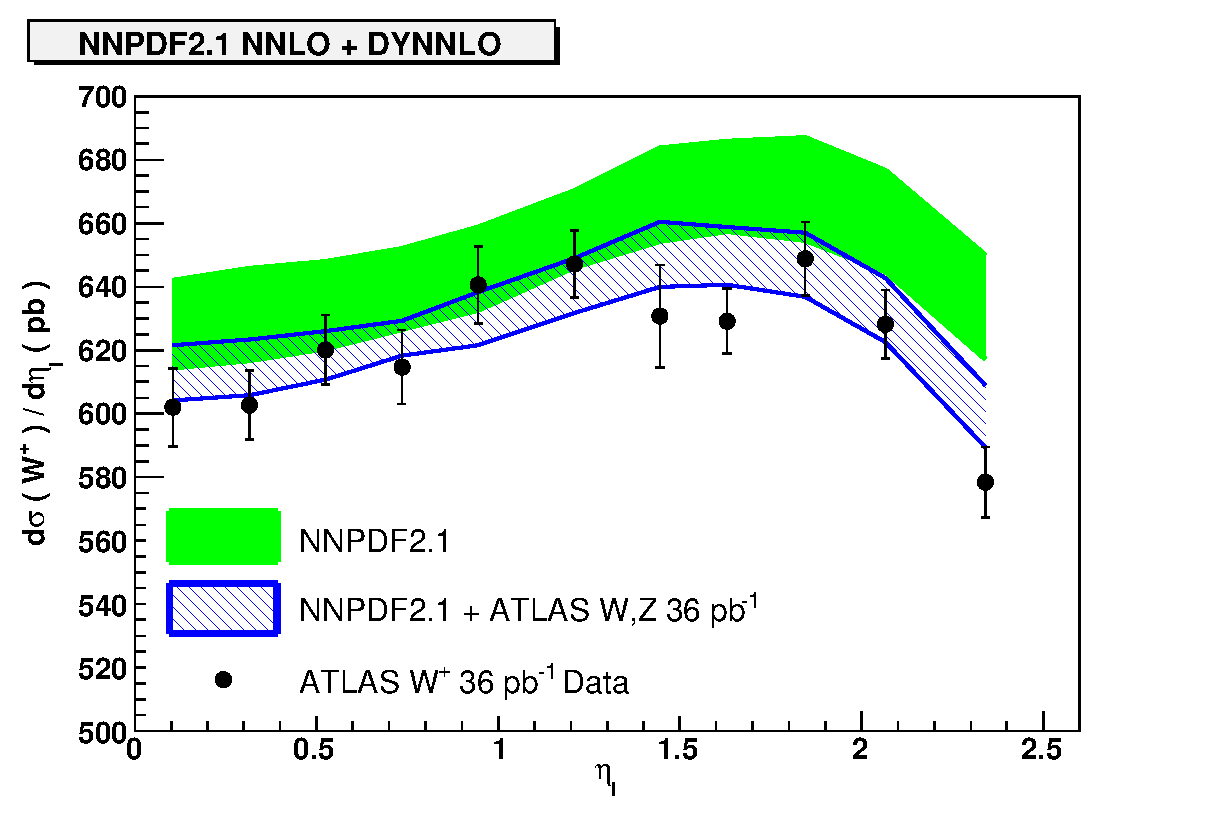
\includegraphics[width=0.52\textwidth]{dat-th-atlaswp}
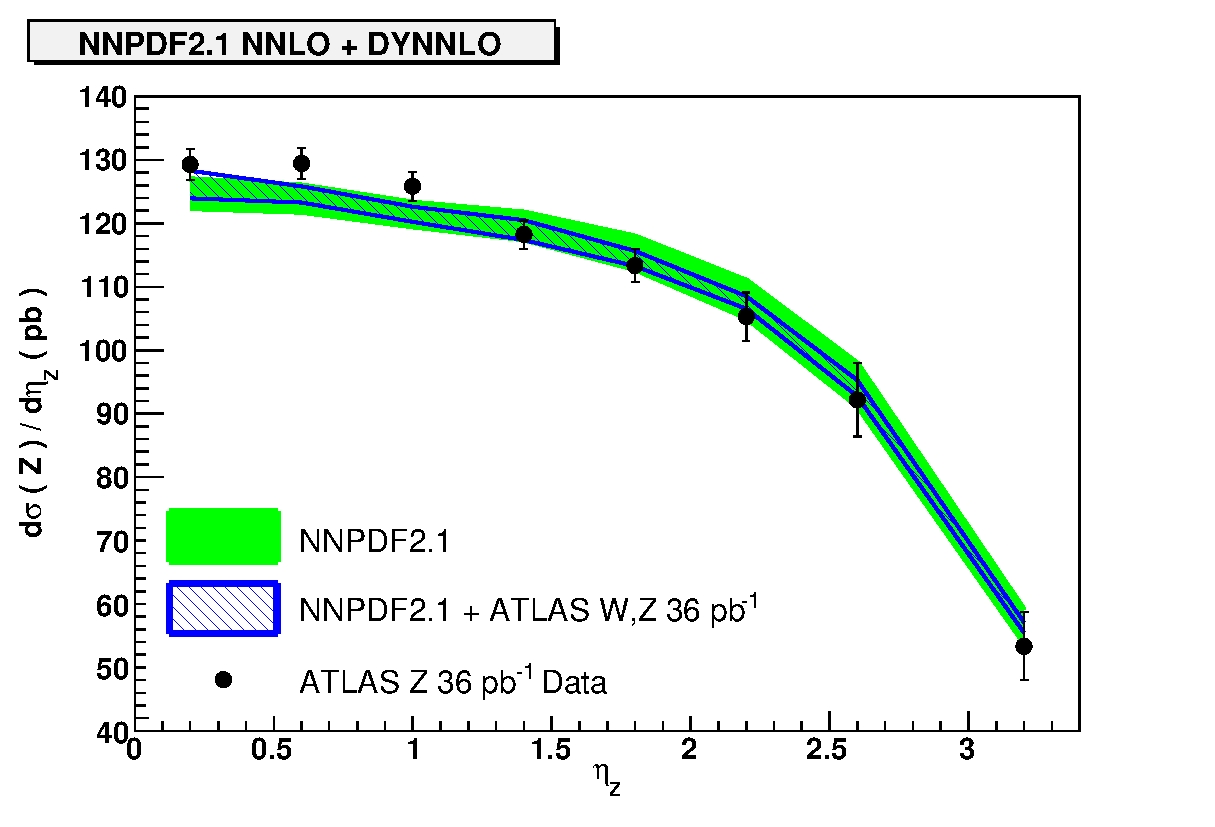
\includegraphics[width=0.52\textwidth]{dat-th-atlasz}\\
\end{center}
\end{frame}

\begin{frame}
\frametitle{Impact of LHC EW vector boson data - CMS}
\textbf{\footnotesize Preliminary reweighting results}
\begin{table}[h]
\scriptsize
\begin{center}
\begin{tabular}{|c|c|c|c|c|}
\hline
Dataset  &  $\chi^2$  &  $\chi^2_{\rm rw} $ & $N_{\rm eff}$  \\
\hline
\hline
CMS  & 2.0       & 1.2   &  56   \\  
\hline
CMS Z rapidity 36 pb$^{-1}$  &    1.9    & 1.4  &  223  \\  
CMS muon asymmetry 234 pb$^{-1}$      &  2.0   & 0.4   & 200   \\  
\hline
\end{tabular}
\end{center}
\end{table}
\begin{center}
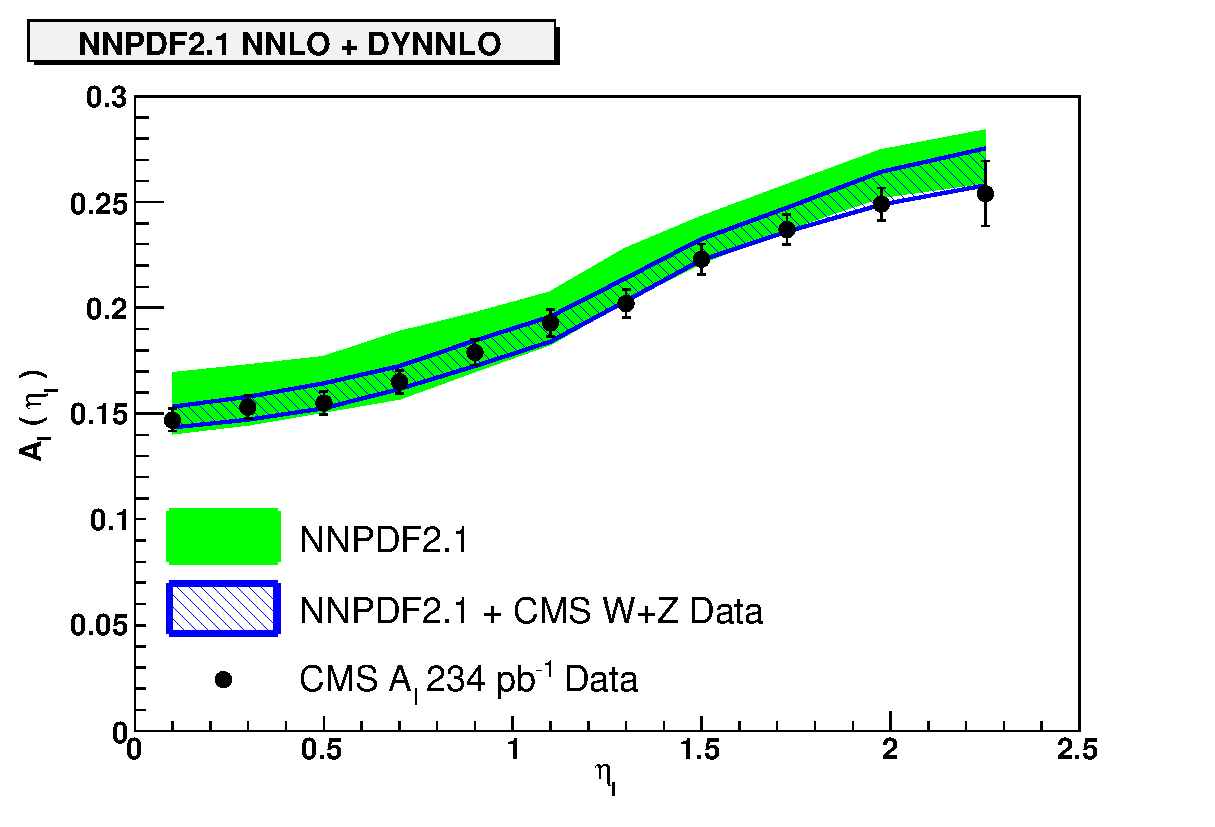
\includegraphics[width=0.52\textwidth]{dat-th-cmswlasy}
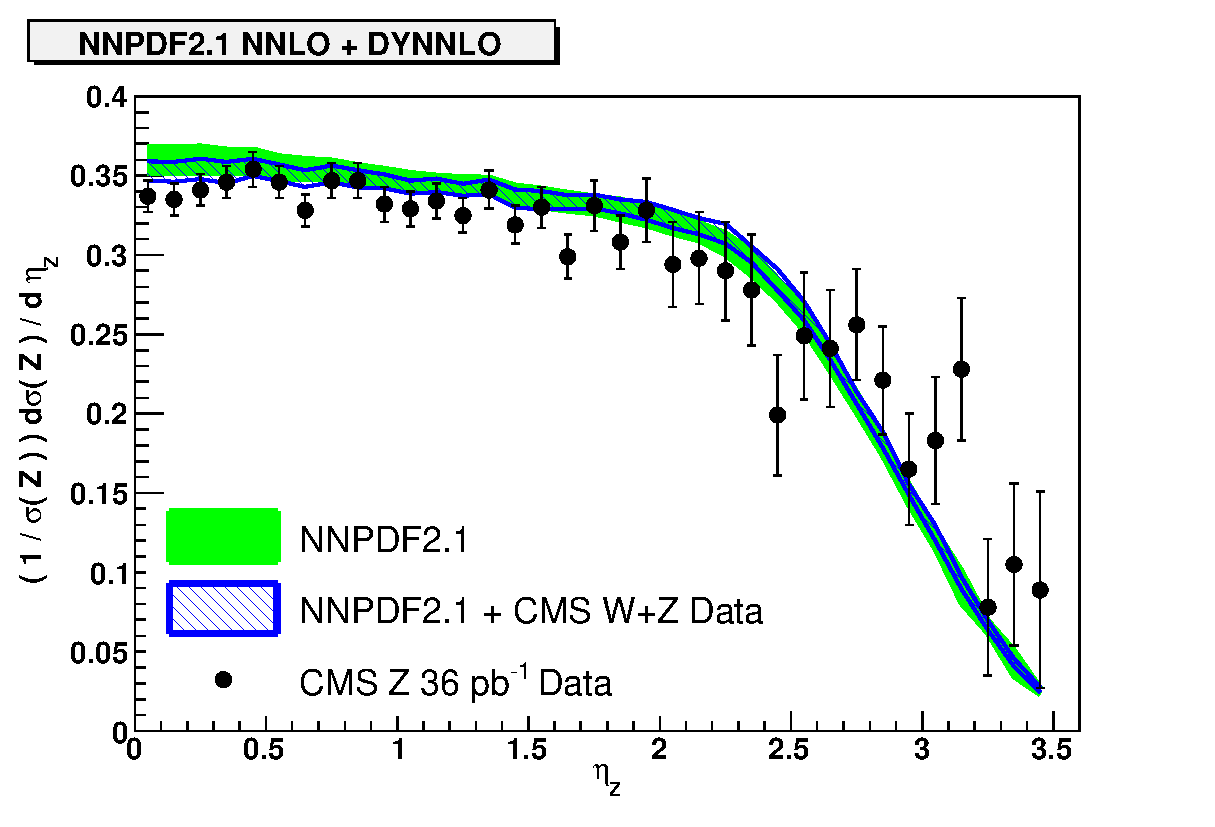
\includegraphics[width=0.52\textwidth]{dat-th-cmsz}\\
\end{center}
\end{frame}

\begin{frame}
\frametitle{Impact of LHC EW vector boson data - LHCb}
\textbf{\footnotesize Preliminary reweighting results}
\begin{table}[h]
\scriptsize
\begin{center}
\begin{tabular}{|c|c|c|c|c|}
\hline
Dataset  &  $\chi^2$  &  $\chi^2_{\rm rw} $ & $N_{\rm eff}$  \\
\hline
\hline
LHCb   &   0.8 & 0.8   & 972    \\ 
\hline
LHCb Z rapidity 36 pb$^{-1}$      &  1.1  & 1.0  & 962   \\  
LHCb  $W$ lepton asymmetry 36 pb$^{-1}$      & 0.8   & 0.5  & 961   \\  
\hline
\end{tabular}
\end{center}
\end{table}
\begin{center}
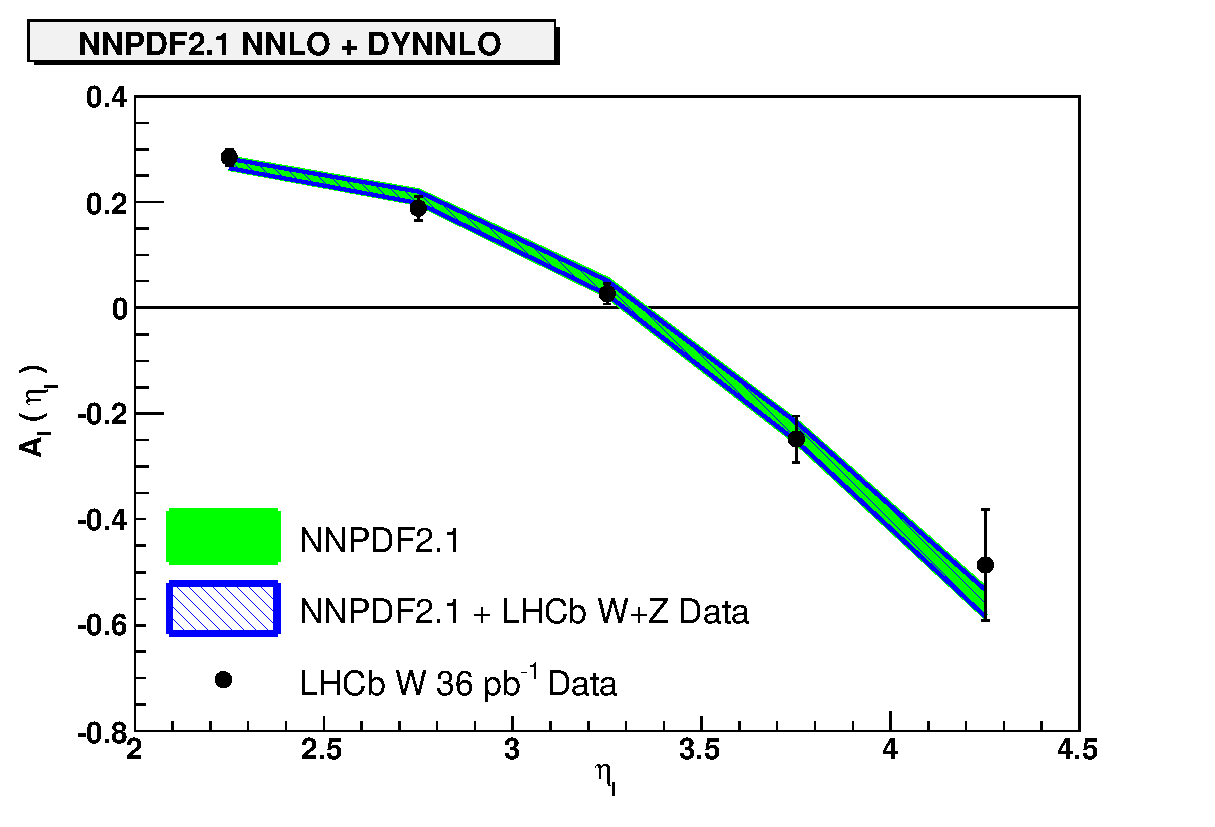
\includegraphics[width=0.52\textwidth]{dat-th-lhcbw}
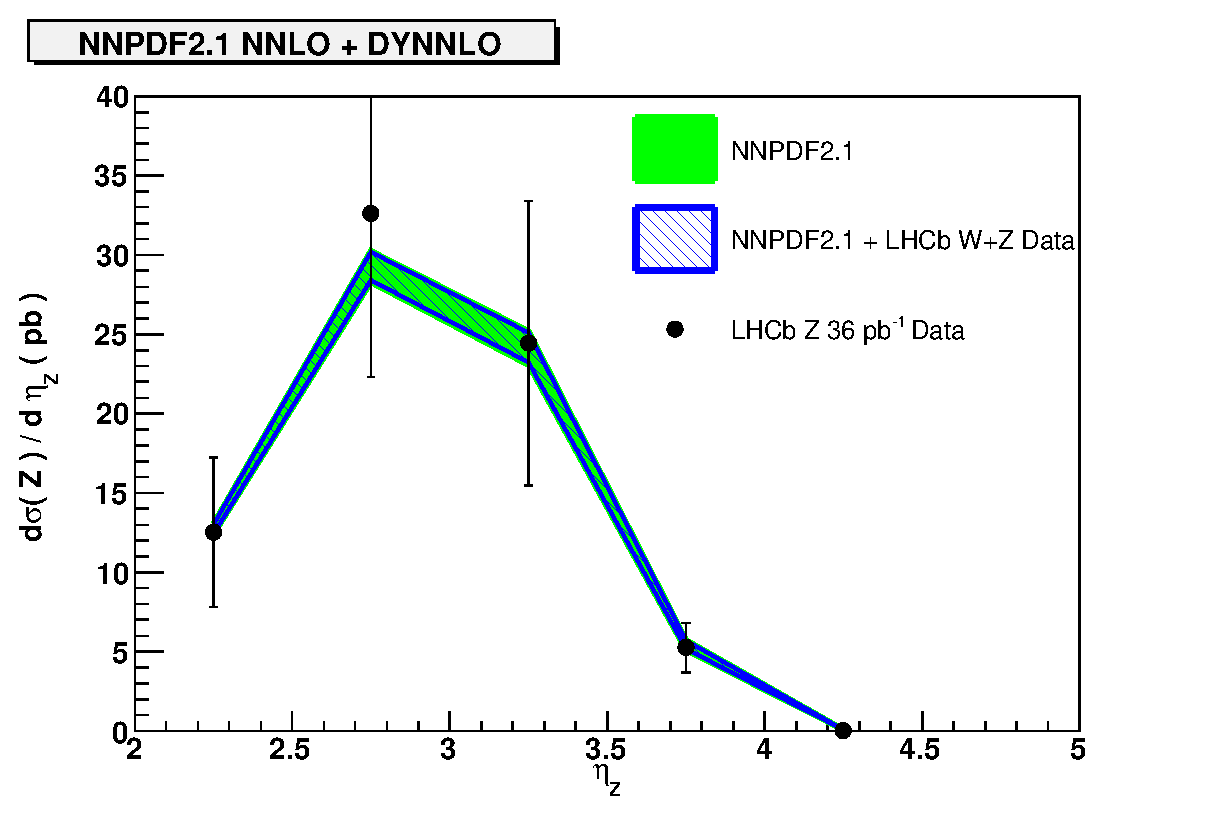
\includegraphics[width=0.52\textwidth]{dat-th-lhcbz}\\
\end{center}
\end{frame}

\begin{frame}
\frametitle{Impact of LHC EW vector boson data}
\begin{centering}
\small Ratio of $d$, $\bar{u}$ PDFs reweighted with ATLAS data to NNPDF2.1\\
\end{centering}
\begin{figure}[h]
\begin{center}
\includegraphics[width=0.40\textwidth]{xd_Q2_10000_log-atlas.eps}
\includegraphics[width=0.40\textwidth]{xubar_Q2_10000_log-atlas.eps}\\
\end{center}
\end{figure}
\begin{centering}
\small Ratio of $d$, $\bar{u}$ PDFs reweighted with CMS data to NNPDF2.1\\
\end{centering}

\begin{figure}[h]
\begin{center}
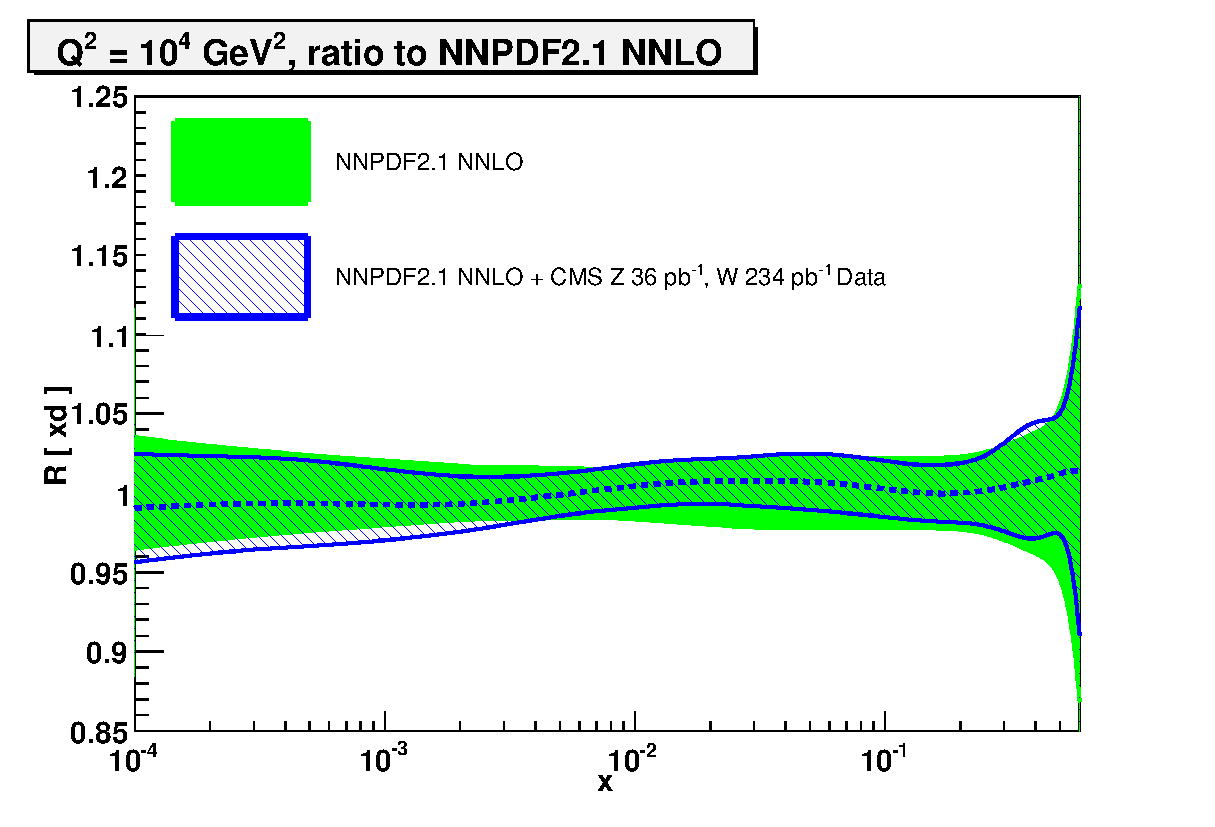
\includegraphics[width=0.40\textwidth]{xd_Q2_10000_log-cms.eps}
\includegraphics[width=0.40\textwidth]{xubar_Q2_10000_log-cms.eps}
\end{center}
\end{figure}

\end{frame}


\begin{frame}
\frametitle{Impact of ATLAS inclusive jet data}
\textbf{\footnotesize Preliminary reweighting results}


\begin{table}[h]
\small
\begin{center}
\begin{tabular}{|c|c|c|c|}
\hline
Dataset  &  $\chi^2$  &  $\chi^2_{\rm rw} $ & $N_{\rm eff}$  \\
\hline
NNPDF2.1 NNLO + ATLAS Incl. Jets     $R=0.4$   & 0.93  & 0.91 & 904       \\  
NNPDF2.1 NNLO + ATLAS Incl. Jets    $R=0.6$   & 1.42  & 1.24 &  610     \\  
\hline
\end{tabular}
\end{center}

\end{table}


\begin{figure}[h!]
  \centering
  \epsfig{width=0.8\textwidth,figure=xg_Q2_10000_lin-atlasR.eps}
\end{figure}

\end{frame}
 
\begin{frame}
\frametitle{Summary}

\begin{itemize}
\item<1-> NNPDF Parton Sets
\begin{itemize}\footnotesize
		\item<1-> Neural Network parametrisation of PDFs. \\
		{ \color{blue} Redundant parametrisation for an unbiased fit.}
		\item<1-> Monte Carlo uncertainty determination.\\
		{ \color{blue}Faithful representation of the experimental uncertainties.}
		\end{itemize}
\item<1-> Bayesian Reweighting
\begin{itemize}\footnotesize
		\item<1-> Powerful technique for including new data into existing parton fits. \\
		{ \color{blue} Fast assessment of data impact.}
		\end{itemize}
\item<1-> Impact of LHC data
\begin{itemize}\footnotesize
		\item<1-> ATLAS $W/Z$ measurements:\\
		{ \color{blue} Substantial constraints, particularly from $W^{+}$ data.}

		\item<1-> CMS $W/Z$ measurements:\\
		{ \color{blue}  Less constraining $\to$ full covariance matrix is unavailable.}\\
		\item<1-> LHCb $W/Z$ measurements:\\
		 { \color{blue} Data does not yet provide significant constraint upon PDFs.}\\
		
		\item<1-> ATLAS inclusive jet measurements:\\
		{ \color{blue} Moderate constraint upon gluon PDF.}

		\end{itemize}
\end{itemize}
\begin{centering}
\textbf{ LHC data already providing significant constraints on parton distributions.}\\
\end{centering}

\end{frame}

\begin{frame}
    \begin{center}
      BACKUPS
    \end{center}
\end{frame}

\begin{frame}
\frametitle{ATLAS Determination of $R_s$}
\begin{centering}
\small Ratio of strange to non-strange PDFs from a HERA + ATLAS W/Z production fit.\\
\end{centering}
\begin{columns}
  \begin{column}{0.5\textwidth}
  \epsfig{width=1\textwidth,figure=ATLAS-rs.pdf}
  \end{column}
    \begin{column}{0.5\textwidth}
   \epsfig{width=1\textwidth,figure=NNPDF-rs.eps}
       \begin{itemize}
		\item<1-> No discrepancy observed with Rs for NNPDF collider +W/Z only fit
\end{itemize}
   \end{column}
  \end{columns}
\end{frame}

\begin{frame}
\frametitle{NNPDF2.1NLO/NNLO reweighted with ATLAS jets}
\begin{figure}[h]
\begin{center}
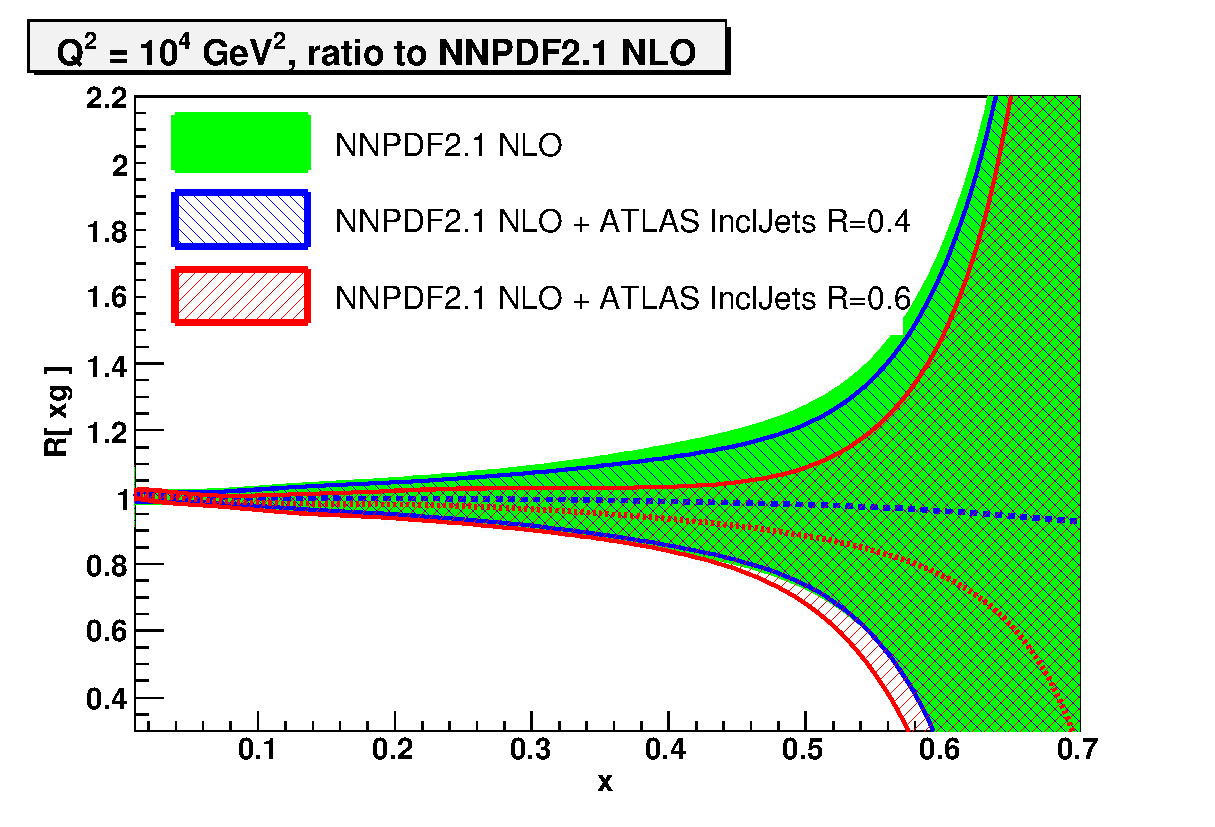
\includegraphics[width=0.49\textwidth]{xg_Q2_10000_lin-atlasnloR.eps}
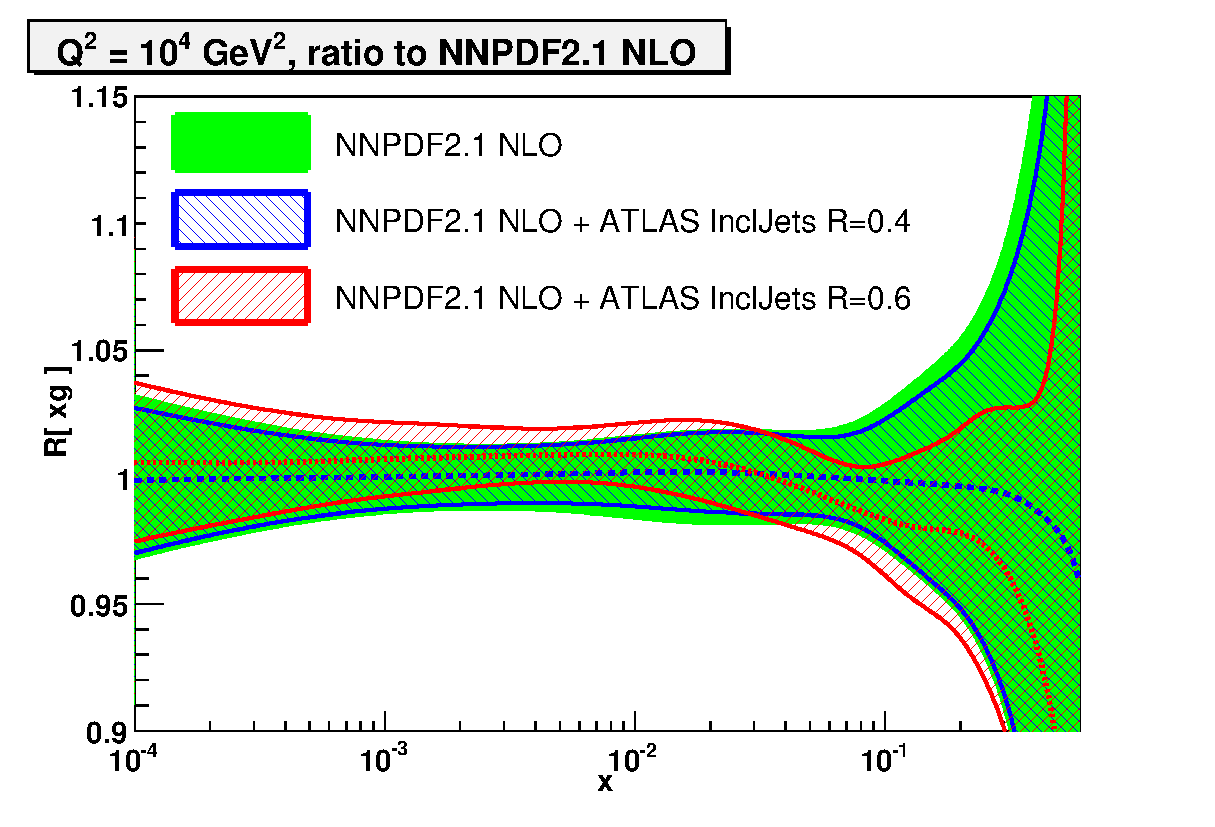
\includegraphics[width=0.49\textwidth]{xg_Q2_10000_log-atlasnloR.eps}\\
\includegraphics[width=0.49\textwidth]{xg_Q2_10000_lin-atlasR.eps}
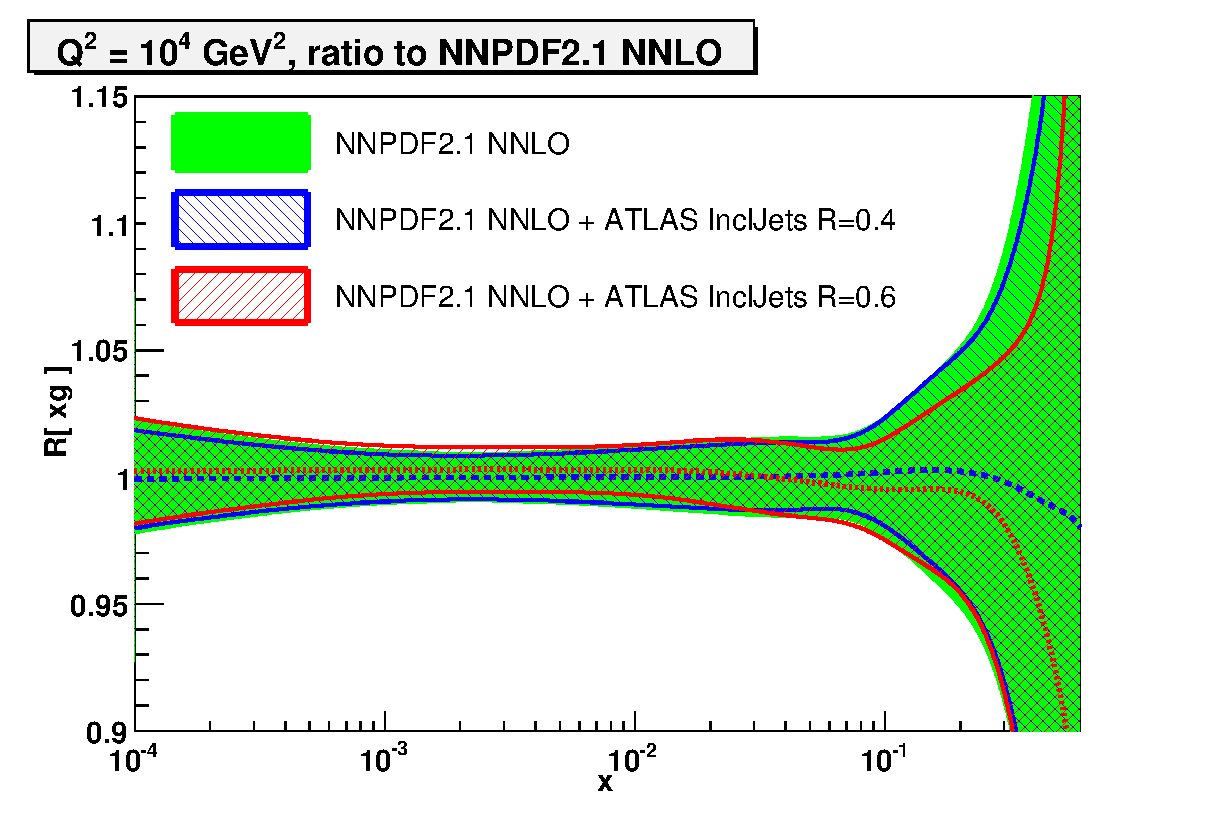
\includegraphics[width=0.49\textwidth]{xg_Q2_10000_log-atlasR.eps}
\label{pdfcomp-jets}
\end{center}
\end{figure}
\end{frame}

%
%
%
%\begin{frame}
%\small
%\frametitle{Special features of NNPDF approach}
%\textbf{Minimisation by genetic algorithms}\\
%\underline{Problem}: Very large parameter space, $\chi2$ highly nonlocal. \begin{itemize}
%\item<1-> Minimisation is challenging.
%\end{itemize}\underline{Solution}: Genetic Algorithms (GA)
%\begin{itemize}
%\item<1-> Generate mutations of fit parameters.
%\item<1-> Select those mutations that minimise figure of merit.
%\end{itemize}
%\vskip10pt
%\textbf{ Dynamical fit stopping by cross-validation}\\
%\underline{Problem}:  extremely flexible parameterisations are prone to \emph{overfitting}.
%\\
%\begin{itemize}
%\item<1->Fit has so many parameters, the minimum $\chi^2$ corresponds to a fit not only to
%the data, but also statistical noise.
%\end{itemize}
%\underline{Solution}:  dynamical stopping by \emph{Cross Validation}.
%\begin{itemize}
%\item<1-> Split the dataset into a training set and a validation set.
%\item<1-> Use the training set for minimisation, monitor the $\chi^2$ to the validation set.
%\item<1-> Stop the fit when the $\chi^2$ to the validation set starts to increase while
%the $\chi^2$ to training set is still decreasing.
%
%\end{itemize}
%
%
%
%\end{frame}
%
%\begin{frame}
%\frametitle{Cross Validation}
% \begin{figure}[b!]
%    \begin{center}
%      \includegraphics[width=0.9\textwidth]{chi2ite-1004-NMC-pd.eps}
%    \end{center}
%\end{figure}
%\end{frame}
%
%\begin{frame}
%\frametitle{Unweighting procedure}
%\begin{columns}
%  \begin{column}{0.5\textwidth}
%\begin{figure}
%  \epsfig{width=0.7\textwidth,figure=unwplot-1.eps,angle=-90}\\
%\end{figure}
%  \end{column}
%  \begin{column}{0.5\textwidth}
%\begin{figure}
%  \epsfig{width=0.7\textwidth,figure=unwplot-2.eps,angle=-90}
%\end{figure}
%  \end{column}
%\end{columns}
%\end{frame}
%

% End of slides
\end{document} 